% Этот шаблон документа разработан в 2014 году
% Данилом Фёдоровых (danil@fedorovykh.ru) 
% для использования в курсе 
% <<Документы и презентации в \LaTeX>>, записанном НИУ ВШЭ
% для Coursera.org: http://coursera.org/course/latex .
% Исходная версия шаблона --- 
% https://www.writelatex.com/coursera/latex/2
\documentclass[../main.tex]{subfiles}

%%% Работа с русским языком
\usepackage{cmap}					% поиск в PDF
\usepackage{mathtext} 				% русские буквы в формулах
\usepackage[T2A]{fontenc}			% кодировка
\usepackage[utf8]{inputenc}			% кодировка исходного текста
\usepackage[english,russian]{babel}	% локализация и переносы

%%% Дополнительная работа с математикой
\usepackage{amsfonts,amssymb,amsthm,mathtools} % AMS
\usepackage{amsmath}
\usepackage{icomma} % "Умная" запятая: $0,2$ --- число, $0, 2$ --- перечисление

%% Номера формул
%\mathtoolsset{showonlyrefs=true} % Показывать номера только у тех формул, на которые есть \eqref{} в тексте.
%% Шрифты
\usepackage{euscript}	 % Шрифт Евклид
\usepackage{mathrsfs} % Красивый матшрифт

%% Свои команды
\DeclareMathOperator{\sgn}{\mathop{sgn}}

%% Перенос знаков в формулах (по Львовскому)
\newcommand*{\hm}[1]{#1\nobreak\discretionary{}
	{\hbox{$\mathsurround=0pt #1$}}{}}

%%% Работа с картинками
\usepackage{graphicx}  % Для вставки рисунков
\graphicspath{{images/1/}{images/2/}{{images/4/}}}  % папки с картинками
\setlength\fboxsep{3pt} % Отступ рамки \fbox{} от рисунка
\setlength\fboxrule{1pt} % Толщина линий рамки \fbox{}
\usepackage{wrapfig} % Обтекание рисунков и таблиц текстом

%%% Работа с таблицами
\usepackage{array,tabularx,tabulary,booktabs} % Дополнительная работа с таблицами
\usepackage{longtable}  % Длинные таблицы
\usepackage{multirow} % Слияние строк в таблице


\usepackage{indentfirst}
\usepackage{hyperref}
\usepackage{booktabs}
\usepackage{float}
\usepackage[table]{xcolor}

% код в matlab
\usepackage{matlab-prettifier}
\usepackage{listings,lstautogobble}
\lstset{autogobble=true}




\begin{document} % конец преамбулы, начало документа
	\subsection{Описание алгоритма имитации отжига}
	Приведем описание алгоритма имитации отжига, который используется для минимизации некоторой функции $H: S \rightarrow \mathbb{R}$.
	\begin{enumerate}
		\item Фиксируется начальное значение температуры $T_0$, а также счетчик $k = 0$. 
		\item Выбирается случайный элемент $s_0 \in S$.
		\item  Понижается температура $T_{k+1} = \alpha T_k, \alpha \in (0, 1)$.
		\item Строится новый элемент $\tilde{s_k} = G(s_k)$, где $G: S \rightarrow S$ - фиксированная исследователем случайная функция.
		\item Вычисляется $\Delta = H(\tilde{s_k}) - H(s_k)$. 
		\item Если $\Delta < 0$, то $s_{k+1} = \tilde{s_k}$. В противном случае с вероятностью $p = \exp{(-\frac{\Delta}{T_k})}$ полагается, что $s_{k+1} = \tilde{s_k}$. С вероятностью $1 - p$  $s_{k+1} = s_k$.
		\item Полагается $k := k + 1$, переход к шагу 3.
		
	\end{enumerate}
	
	
	\subsection{Задача о расстановке ферзей}
	В данной главе будет решаться задача расстановки $n$ ферзей на шахматной доске размера $n\times n$ так, чтобы они друг друга не били. Для решения задачи будет минимизироваться количество различных упорядоченных пар бьющих друг друга ферзей с использованием алгоритма имитации отжига. 
	
	В качестве кодировки расстановки ферзей будет использован одномерный массив из $n$ элементов, каждый из которых отвечает за номер горизонтали позиции соответствующего ферзя. Заметим, что для того, чтобы ферзи не били друг друга, необходимо, чтобы они стояли на разных вертикалях и горизонталях, поэтому искомая расстановка является перестановкой элементов множества $\{1, \dots, n\}$.
	
	Сначала требуется написать функцию, которая будет по расстановке ферзей считать количество упорядоченных пар бьющих друг друга ферзей. Идея алгоритма подсчета в том, что мы будем проходиться по всем парам ферзей и считать эту пару 'бьющей', если модуль разности номеров строк и столбцов позиций ферзей одинаковы. Таким образом, код этой функции в MATLAB имеет следующий вид:
	
	
	\begin{lstlisting}[
		frame=single,
		numbers=left,
		style=Matlab-Pyglike]
		function [cnt] = h(q)
		n = size(q, 2);
		cnt = 0;
		for i = 1:n
		  for j = i+1:n
		    if j - i == abs(q(j) - q(i))
			  cnt = cnt + 2;
		    end
	 	  end
		end
		end
	\end{lstlisting}

	Также требуется написать функцию, которая будет менять местами два случайных элемента массива, ее код будет иметь вид:
	
	\begin{lstlisting}[
		frame=single,
		numbers=left,
		style=Matlab-Pyglike]
		function [q_old] = swap(q_old)
		n = size(q_old, 2);
		idx = randi([1, n], 1, 2);
		q_old([idx(1), idx(2)]) = q_old([idx(2), idx(1)]);
		end
	\end{lstlisting}
	
	Теперь реализуем алгоритм имитации отжига в виде функции, которая на вход будет принимать три параметра: $n$ - размер доски и одновременно количество ферзей, $\alpha$ - множитель, на который умножается температура, $t_0$ - начальная температура. В качестве выхода будет выступать итоговая расстановка ферзей $q$, количество шагов алгоритма $k$ и общее количество итераций. 
	
	Основная идея алгоритма состоит в том, что мы будем менять номера горизонталей двух случайных ферзей местами -  при уменьшении количества бьющих ферзей выберем новую расстановку, в противном случае выберем ее с некоторой вероятностью, которая будет зависеть от прироста целевой функции и постепенно уменьшающейся температуры. Когда будет получена искомая расстановка, процесс остановится. Код функции в MATLAB: 
	
	\begin{lstlisting}[
		frame=single,
		numbers=left,
		style=Matlab-Pyglike]
		function [q, k] = annealing(n, alpha, t_0)
		t = t_0;
		q = 1:n;
		strikes = h(q);
		k = 0;
		while strikes ~= 0
		  t_new = alpha * t;
		  q_new = swap(q);
		  strikes_new = h(q_new);
		  delta_strikes = strikes_new - strikes;
		  p = exp(-delta_strikes / t);
		  xi = binornd(1, p);
		  if or(delta_strikes < 0, xi == 1)
		    q = q_new;
		    strikes = strikes_new;
		  end
		  t = t_new;
		  k = k + 1;
		end
	\end{lstlisting}

	Протестируем полученную программу, для чего рассмотрим случай 8 ферзей и обычной шахматной доски $8\times 8$, в качестве $\alpha$ возьмем 0.8 (значение было подобрано на основании результатов нескольких запусков, минимизируя количество итераций алгоритма), а начальную температуру положим равной 100. Тогда получим следующее:
	
	\begin{lstlisting}[
		frame=single,
		numbers=left,
		style=Matlab-Pyglike]
		>> [q, k] = annealing(8, 0.8, 100)
		
		q =
		
		5     7     1     4     2     8     6     3
		
		
		k =
		
		60
		
		>> 
	\end{lstlisting}
	
	Нетрудно заметить, что в полученой расстановке ферзи не бьют друг друга, продемонстрируем это визуально.
	\begin{figure}[H]
		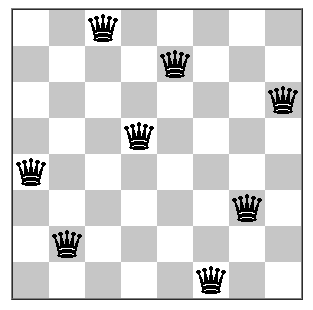
\includegraphics[width = \textwidth / 2]{ann_1}
	\end{figure}
	
	
	Сделаем то же самое, но с 12 ферзями:
	
	\begin{lstlisting}[
		frame=single,
		numbers=left,
		style=Matlab-Pyglike]
		>> [q, k]  = annealing(12, 0.8, 100)
		
		q =
		
		10     7     3     6    11     9     1    12     4     2     8     5
		
		
		k =
		
		628
		
		>>  
	\end{lstlisting}
	
	На этот раз ферзи также не бьют друг друга:
	
	\begin{figure}[H]
		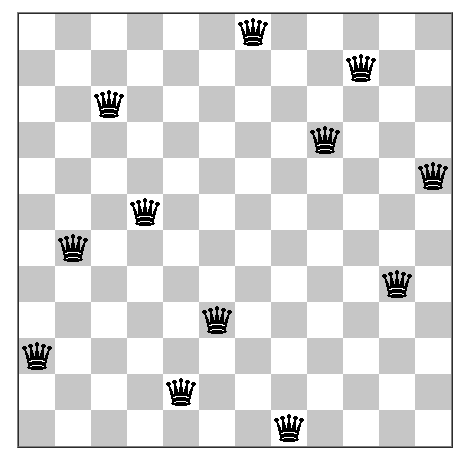
\includegraphics[width = 0.7\textwidth]{ann_2}
	\end{figure}
	
	
	
	Попробуем увеличить размерность задачи и расставим 20 ферзей.
	
	\begin{lstlisting}[
		frame=single,
		numbers=left,
		style=Matlab-Pyglike]
	>> [q, k_0] = annealing(20, 0.8, 100);
	[q, k_1] = annealing(20, 0.8, 100);
	[q, k_2] = annealing(20, 0.8, 100);
	[q, k_3] = annealing(20, 0.8, 100);
	[q, k_4] = annealing(20, 0.8, 100);
	[k_0, k_1, k_2, k_3, k_4]
	
	ans =
	
	499   654   425   467   219
	
	>> 
	\end{lstlisting}
	
	Видно, что количество шагов и итераций достаточно низкое, поэтому можно сказать, что алгоритм достаточно быстро справился с поставленной задачей.
	
	Даже если увеличить количество ферзей до 100, то итераций будет по-прежнему немного.
	
	
		\begin{lstlisting}[
		frame=single,
		numbers=left,
		style=Matlab-Pyglike]
		>> [q, k_0] = annealing(100, 0.8, 100);
		[q, k_1] = annealing(100, 0.8, 100);
		[q, k_2] = annealing(100, 0.8, 100);
		[q, k_3] = annealing(100, 0.8, 100);
		[q, k_4] = annealing(100, 0.8, 100);
		[k_0, k_1, k_2, k_3, k_4]
		
		ans =
		
		6036        3693        5115        8328       12685
		
		>>  
	\end{lstlisting} 
	
	Таким образом, задача по применению метода имитации отжига к решению задачи о расстановке ферзей на шахматной доске так, чтобы они друг друга не били, успешно решена.
	
	
\end{document} % конец документа